% !TeX program = xelatex
\documentclass[12pt]{article}

\usepackage[left=2.5cm,right=2.5cm,top=3cm,bottom=3cm]{geometry}

\usepackage{polyglossia}
\setmainlanguage{russian}
\setotherlanguage{english}

\setmainfont[
SmallCapsFont={Latin Modern Roman Caps},
SmallCapsFeatures={Letters=SmallCaps},
Ligatures=TeX
]{Times New Roman}

\usepackage[intlimits]{amsmath}
\usepackage{amssymb}
\usepackage{mathrsfs}
\usepackage{indentfirst}

\newcommand{\pd}[2]{\frac{\partial #1}{\partial #2}}
\newcommand{\dpd}[2]{\dfrac{\partial #1}{\partial #2}}

\newcommand{\pdd}[2]{\frac{\partial^2 #1}{\partial #2^2}}
\newcommand{\pddd}[3]{\frac{\partial^2 #1}{\partial #2\partial #3}}

\renewcommand{\arraystretch}{1.2}
\let\dividesymbol\div
\renewcommand{\div}{\operatorname{div}}
\newcommand{\grad}{\operatorname{grad}}
\newcommand{\rot}{\operatorname{rot}}
\newcommand{\const}{\operatorname{const}}
\renewcommand{\vec}[1]{\boldsymbol{\mathbf{#1}}}
\newcommand{\ten}[1]{\mathbf{#1}}
\newcommand{\cutefrac}[2]{{}^{#1}\mkern-5mu/{\!}_#2}
\newcommand{\half}{{\cutefrac{1}{2}}}
\renewcommand{\leq}{\leqslant}
\renewcommand{\geq}{\geqslant}

\author{Цыбулин Иван}
\title{Автомодельные решения уравнения теплопроводности}

\begin{document}
\maketitle

\section{Автомодельные решения}

Автомодельными решениями называются такие решения, которые зависят не от $x$ и $t$ в отдельности, а лишь от некоторой их комбинации $\xi = \xi(t, x)$:
\[
u(t, x) = u(\xi(t, x)).
\]
Автомодельные решения называют еще \emph{самоподобными} (\foreignlanguage{english}{\emph{similarity solutions}} или \foreignlanguage{english}{\emph{self-similar solutions}}), так как в них с течением времени решение остается подобным себе в начальный момент времени.

Одно и то же уравнение может иметь автомодельные решения для различных автомодельных переменных. Например, для системы уравнений газовой динамики существуют автомодельные решения вида бегущей волны (с $\xi = x - Dt$)
\begin{gather*}
\rho(t, x) = \rho_0(x - D t)\\
u(t, x) = D\\
\varepsilon(t, x) = \frac{p_0}{(\gamma - 1) \rho_0(x - D t)}
\end{gather*}
для произвольных параметров $p_0, D$ и произвольной функции $\rho_0(\xi)$. Это решение переносится со скоростью $D$, сохраняя свою форму. В задаче Римана (о распаде произвольного разрыва) решение является автомодельным, но уже относительно переменной $\xi = x/t$. Со временем это решение <<растягивается>> вдоль оси $x$.

Не любая комбинация параметров $\xi(t, x)$ может быть автомодельной переменной. Для того, чтобы выяснить, годится ли данная переменная в качестве автомодельной, можно рассмотреть замену переменных
\begin{gather*}
\xi = \xi(t, x)\\
\tau = \tau(t, x) \equiv t.
\end{gather*}
Если после такой замены переменных из уравнений может быть исключена переменная $\tau$, такая переменная $\xi(t, x)$ будет давать автомодельное решение.

\section{Линейное уравнение теплопроводности}
Рассмотрим линейное уравнение теплопроводности
\[
u_t = \lambda u_{xx}, \quad \lambda = \const.
\]

\subsection{Поиск автомодельных решений из соображений размерности}

В неограниченной области решение этого уравнения с известным начальным условием $u(0, x) = \varphi(x)$ может быть найдено с помощью интеграла Пуассона:
\[
u(t, x) = \frac{1}{\sqrt{4 \lambda \pi t}}\int_{-\infty}^{\infty}  \exp\left(
-\frac{(x-y)^2}{4 \lambda t}
\right) \varphi(y) dy
\]

Возможность записать решение уравнения в такой форме напрямую следует из линейности задачи. Функция
\[
\Phi(t, x) = \frac{1}{\sqrt{4\lambda\pi t}} \exp\left(-\frac{x^2}{4\lambda t}\right)
\]
называется \emph{фундаментальным решением} и описывает решение уравнения теплопроводности с точечным начальным распределением температуры
\[
u(x, 0) = \delta(x).
\]
Составляя из точечных распределений заданное начальное условие
\[
u(x, 0) = \varphi(x) = \int_{-\infty}^{\infty} \varphi(y) \delta(x - y) dy
\]
и пользуясь линейностью задачи по начальным данным, получаем решение уравнения в виде
\[
u(t, x) = \int_{-\infty}^{\infty} \varphi(y) \Phi(x-y, t) dy.
\]

Рассмотрим задачу с начальным распределением температуры в виде ступеньки:
\[
\varphi(x) = \begin{cases}
1, &x \leq 0\\
0, &x > 0
\end{cases}.
\]
Решением этой задачи будет
\[
u(t, x) = \frac{1}{\sqrt{4 \lambda \pi t}}\int_{-\infty}^{0}  \exp\left(
-\frac{(x-y)^2}{4 \lambda t}
\right) dy = \frac{1}{2} \operatorname{erfc}\left(\frac{x}{2\sqrt{\lambda t}}\right).
\]
Функция $\operatorname{erfc}$ называется дополнительной функцией ошибок и определяется как
\[
\operatorname{erfc}(z) = \frac{2}{\sqrt{\pi}} \int_{z}^\infty e^{-t^2} dt.
\]
\begin{figure}[ht!]
\centering
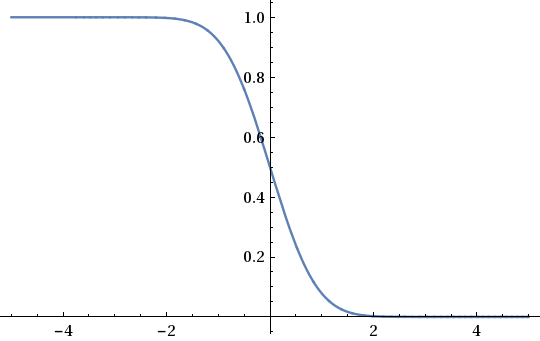
\includegraphics[width=.45\textwidth]{erfc.png}
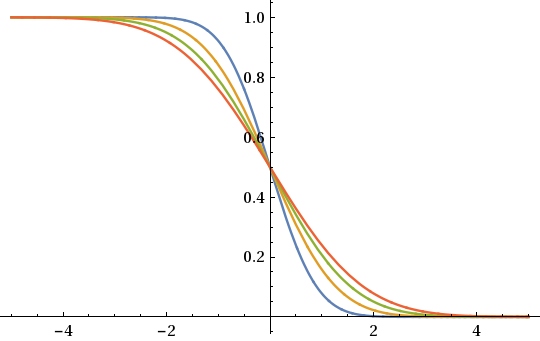
\includegraphics[width=.45\textwidth]{attimes.png}
\caption{Функция $\frac{1}{2}\operatorname{erfc}(\xi)$ (слева) и решение $u(t,x)$ в последовательные моменты времени (справа)}
\end{figure}

Заметим, что решение данной задачи оказалось автомодельным, оно зависит лишь от переменной $\xi = \frac{x}{2\sqrt{\lambda t}}$ и со временем лишь растягивается по закону $\Delta x \sim \sqrt{t}$. Исходная задача не содержала ни масштабов длины (начальное условие содержит единственный разрыв и не имеет характерных размеров), ни масштабов времени (во времени никакие параметры задачи не менялись). Согласно $\pi$-теореме в этом случае решение должно зависеть лишь от безразмерных параметров. Единственным нетривиальным безразмерным параметром данной задачи является именно величина $\xi = \frac{x}{2\sqrt{\lambda t}}, \quad [\lambda] = L^2T^{-1}$.
Исходя из той же $\pi$-теоремы, задача Римана для уравнений газовой динамики должна иметь автомодельное решение с переменной $\xi = \frac{x}{ct}$, где $c$ --- характерная скорость в задаче (например, скорость звука).

\subsection{Поиск подходящей автомодельной переменной}
Найдем это же автомодельное решение линейного уравнения теплопроводности, но исходя лишь из вида автомодельной переменной $\xi = \frac{x}{t^\alpha}$ ($\alpha$ пока не известно). Проведем замену переменных
\begin{gather*}
\xi = \frac{x}{t^\alpha}\\
\tau = t.
\end{gather*}
Соответственно,
\begin{gather*}
\pd{}{t} = \pd{\xi}{t}\pd{}{\xi} + \pd{\tau}{t}\pd{}{\tau} = \pd{\xi}{t}\pd{}{\xi} + \pd{}{\tau}\\
\pd{}{x} = \pd{\xi}{x}\pd{}{\xi} + \pd{\tau}{x}\pd{}{\tau} = \pd{\xi}{x}\pd{}{\xi}
\end{gather*}
Для случая $\xi = xt^{-\alpha}$
\begin{gather*}
\pd{}{t} = -\frac{\alpha x}{t^{\alpha+1}}\pd{}{\xi} + \pd{}{\tau} = 
-\frac{\alpha \xi}{\tau} \pd{}{\xi} + \pd{}{\tau}
\\
\pd{}{x} = \frac{1}{t^\alpha}\pd{}{\xi} = \frac{1}{\tau^\alpha} \pd{}{\xi}
\end{gather*}
Уравнение теплопроводности в новых переменных $\xi, \tau$ представляется в виде
\[
-\frac{\alpha \xi}{\tau} u_\xi + u_\tau = \lambda \frac{1}{\tau^\alpha} \pd{}{\xi}\left(
\frac{1}{\tau^\alpha} u_\xi
\right) = 
\frac{\lambda}{\tau^{2\alpha}} u_{\xi\xi}.
\]
Это уравнение полностью эквивалентно исходному. Нам интересно, имеет ли это уравнение решение в виде
\[
u(\tau, \xi) = u(\xi).
\]
При этом $u_\tau \equiv 0$ и $u$ должна удовлетворять уравнению
\[
-\frac{\alpha \xi}{\tau} u_\xi = 
\frac{\lambda}{\tau^{2\alpha}} u_{\xi\xi}.
\]
Решение этого уравнения не зависит от $\tau$ в двух случаях
\begin{itemize}
\item $\alpha = 0, \xi = x$. При этом $u_{\xi\xi} = 0$, 
\[u(t, x) = u(\xi) = C_1\xi+C_2 = C_1 x + C_2.\]
Это стационарное (не зависящее от времени) решение уравнения теплопроводности.
\item $\alpha = \frac{1}{2}, \xi = \frac{x}{\sqrt{t}}$. Разберем этот случай подробнее.
\end{itemize}
Решение удовлетворяет уравнению
\[
-\frac{\xi}{2} u_\xi = \lambda u_{\xi\xi}
\]
Относительно $v = u_\xi$ в этом уравнении разделяются переменные
\begin{gather*}
-\frac{\xi d\xi}{2} = \lambda \frac{dv}{v}\\
v(\xi) = C_1 e^{-\xi^2/(4\lambda)}\\
u(\xi) = C_2 + C_1 \int_{-\infty}^{\xi} e^{-t^2/(4\lambda)} dt = 
\tilde{C}_1 \operatorname{erfc}\left(\frac{\xi}{2\sqrt{\lambda}}\right) + \tilde{C}_2
\end{gather*}
Таким образом, мы получили автомодельное решение уравнения теплопроводности для переменной $\xi = \frac{x}{\sqrt{t}}$:
\[
u(t, x) = \tilde{C}_1 \operatorname{erfc}\left(\frac{x}{2\sqrt{\lambda t}}\right) + \tilde{C}_2
\]
С точностью до умножения на число и добавления константы это решение совпадает с решением о распаде температурной ступеньки, полученным из интеграла Пуассона.

\subsection{Решения вида бегущей волны}
Проделаем те же действия, но для другой автомодельной переменной
\[
\xi = x - D t, \quad (\tau = t)
\]
Аналогично, заменяя переменные
\begin{gather*}
\pd{}{t} = \pd{\xi}{t} \pd{}{\xi} + \pd{}{\tau} = -D\pd{}{\xi} + \pd{}{\tau}\\
\pd{}{x} = \pd{\xi}{x} \pd{}{\xi} = \pd{}{\xi},
\end{gather*}
получаем уравнение в виде
\[
-D u_\xi + u_\tau = \lambda u_{\xi\xi}.
\]
Так как нас интересуют решения $u = u(\xi)$ избавляемся от $u_\tau$:
\[
-D u_\xi = \lambda u_{\xi\xi}.
\]
Это уравнение имеет решения при любой $D$. Решением данного уравнения с постоянными коэффициентами будет
\begin{gather*}
u(\xi) = C_1 + C_2 e^{-\frac{D \xi}{\lambda}}\\
u(t, x) = C_1 + C_2 \exp\left(-\frac{D}{\lambda}(x - D t)\right).
\end{gather*}
Отметим, что решение является функцией безразмерной величины $\zeta$
\[
\zeta = \frac{D}{\lambda}(x - D t), \quad [D] = LT^{-1}, [\lambda] = L^2T^{-1}.
\]
Решение представляет собой экспоненциальный профиль, движущийся вправо со скоростью $D$.

\section{Нелинейное уравнение теплопроводности}

Рассмотрим теперь уравнение теплопроводности с коэффициентом теплопроводности, зависящем от решения степенным образом:
\[
T_t = (\lambda(T) T_x)_x, \quad \lambda(T) = \lambda_0 \left(\frac{T}{T_0}\right)^k, \quad k > 0.
\]
В этом уравнении $\lambda_0 = \const$ --- коэффициент теплопроводности при $T = T_0 = \const$. Пусть $u = \frac{T}{T_0}$ --- безразмерная температура ($[u] = 1$). Тогда
\[
u_t = \lambda_0 (u^k u_x)_x.
\]
В этом нелинейном уравнении не работает принцип суперпозиции решений, то есть линейная комбинация двух решений этого уравнения не является решением уравнения. Соответственно, для данного уравнения нет формул типа интеграла Пуассона.

Будем строить для данного уравнения автомодельные решения рассматривая различные автомодельные переменные.

\subsection{Решение вида бегущей волны}
Возьмем
\begin{gather}
\xi = x - D t\\
\tau = t.
\end{gather}
Тогда
\begin{gather*}
\pd{}{t} = \pd{\xi}{t} \pd{}{\xi} + \pd{}{\tau} = -D\pd{}{\xi} + \pd{}{\tau}\\
\pd{}{x} = \pd{\xi}{x} \pd{}{\xi} = \pd{}{\xi},
\end{gather*}
а уравнение принимает вид
\[
-Du_\xi + u_\tau = \lambda_0(u^k u_\xi)_\xi.
\]
Учтем, что мы ищем решения вида $u = u(\xi)$, и $u_\tau = 0$:
\[
-Du_\xi = \lambda_0(u^k u_\xi)_\xi.
\]
Общее решение для этого уравнения довольно сложно. Найдем частное решение, произведя подстановку $u = (A \xi)^n$, при этом
\begin{gather*}
-Dn A^n \xi^{n-1} = \lambda_0 A^{kn+n} n (kn+n-1) \xi^{kn+n-2}\\
-D = \lambda_0 A^{kn} (kn+n-1) \xi^{kn-1}
\end{gather*}
В этом равенстве неизвестными величинами являются $n$ и $A$, а величина $\xi$ пробегает всевозможные значения. Единственным вариантом, когда это равенство станет тождеством, является случай
\[
kn = 1, \quad -D = \lambda_0 A n.
\]
Таким образом, при 
\[
n = \frac{1}{k}, \quad A = -\frac{Dk}{\lambda_0}
\]
уравнение имеет решение в виде $u = (A\xi)^n$
\begin{gather*}
u(\xi) = \sqrt[k]{-\frac{Dk}{\lambda_0}\xi}\\
u(t, x) = \sqrt[k]{\frac{Dk}{\lambda_0}(D t - x)}.
\end{gather*}
Данное решение существует лишь в области $x < Dt$, в остальной области его можно доопределить $u \equiv 0$. Такое доопределение требует обоснования, в частности необходимо показать, что в точке <<сшивания>> $x = Dt$ величина $u^k u_x$ остается непрерывной. В данном случае это условие выполнено.
\begin{figure}[ht!]
\centering
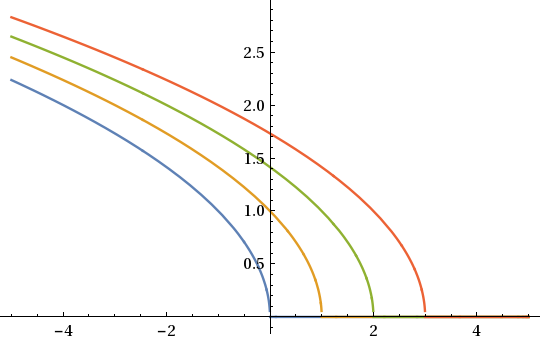
\includegraphics[width=.5\textwidth]{const.png}
\caption{Автомодельное решение в виде бегущей волны в различные моменты времени для $k = 2$}
\end{figure}

\subsection{Решение с переменной $\xi = xt^{-\alpha}$}
Исследуем случай переменной $\xi = xt^{-\alpha}$:
\begin{gather*}
\xi = \frac{x}{t^\alpha}\\
\tau = t.
\end{gather*}
\begin{gather*}
\pd{}{t} = -\frac{\alpha \xi}{\tau} \pd{}{\xi} + \pd{}{\tau}
\\
\pd{}{x} = \frac{1}{\tau^\alpha} \pd{}{\xi}
\end{gather*}
Записывая уравнение и избавляясь от $u_\tau$, получаем
\[
-\frac{\alpha \xi}{\tau} u_\xi = \frac{\lambda_0}{\tau^{2\alpha}}(u^k u_\xi)_\xi.
\]
Из этого уравнения исключается $\tau$ при $\alpha = 0$ и при $\alpha = \frac{1}{2}$.

Для $\alpha = 0$ получается стационарное решение $u(t, x) = u(x)$
\begin{gather*}
u(\xi) = \sqrt[k+1]{C_1 \xi + C_2}\\
u(t, x) = \sqrt[k+1]{C_1 x + C_2}.
\end{gather*}

Для $\alpha = \frac{1}{2}$ получается следующее уравнение для $u(\xi)$:
\[
-\frac{\xi}{2}u_\xi = \lambda_0 (u^k u_\xi)_\xi
\]
Общее решение этого уравнения не выражается в элементарных функциях. Тем не менее, любое решение этого уравнения задает некоторое автомодельное решение $u(t, x)$.

Например, дополнив это уравнение двумя условиями
\begin{gather*}
-\frac{\xi}{2}u_\xi = \lambda_0 (u^k u_\xi)_\xi\\
u\big|_{\xi = 0} = 1, \qquad u\big|_{\xi = \infty} = 0
\end{gather*}
можно получить единственное решение, соответствующее задаче для исходного уравнения теплопроводности с граничными условиями
\begin{gather*}
u\big|_{x = 0} = 1, \qquad u\big|_{x = \infty} = 0.
\end{gather*}
Эта постановка имеет смысл прогрева полупространства с постоянной температурой на границе.
\begin{figure}[ht!]
\centering
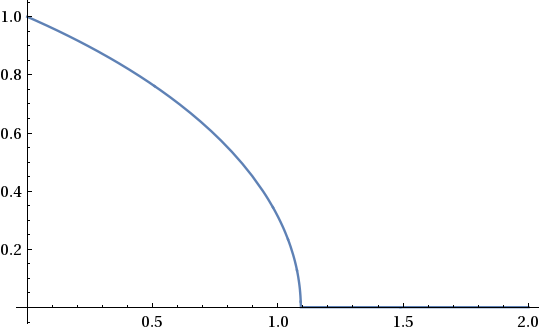
\includegraphics[width=.45\textwidth]{heating.png}
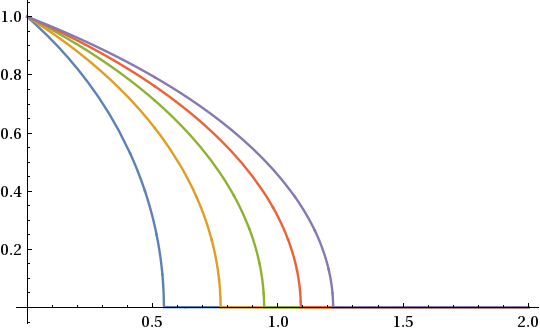
\includegraphics[width=.45\textwidth]{heattimes.png}
\caption{Функция $u(\xi)$ (слева) и решение $u(t,x)$ в последовательные моменты времени (справа) для задачи о прогреве полупространства в случае $k = 2$}
\end{figure}

Другое решение можно получить, как и ранее, подстановкой в виде $u = (A\xi)^{n}$
\begin{gather*}
-\frac{n}{2} A^n \xi^{n} = \lambda_0 A^{kn+n} n (kn+n-1) \xi^{kn+n-2}\\
-\frac{1}{2} = \lambda_0 A^{kn} (kn+n-1) \xi^{kn-2}
\end{gather*}
Равенство превращается в тождество при 
\[
n = \frac{2}{k}, \qquad A^2 = -\frac{k}{2\lambda_0 (k+2)}
\]
При этом получается решение $u(t, x)$ в виде
\[
u = \sqrt[k]{-\frac{kx^2}{2\lambda_0(k+2)t}}.
\]
Это решение имеет смысл лишь при $t < 0$.
Рассмотрим решение, получающееся из него простым сдвигом начального момента времени:
\[
t \to t - t_0
\]
\[
u = \sqrt[k]{\frac{kx^2}{2\lambda_0(k+2)(t_0 - t)}}.
\]
Это решение существует лишь до момента времени $t < t_0$, а затем обращается в бесконечность. Аналогично сдвигу времени, можно произвести сдвиг оси $x$:
\[
u = \sqrt[k]{\frac{k(x-x_0)^2}{2\lambda_0(k+2)(t_0 - t)}}.
\]
По сути, данные сдвиги меняют автомодельную переменную
\[
\xi = \frac{x}{\sqrt{t}} \to \xi = \frac{x-x_0}{\sqrt{t - t_0}}
\]
сдвигая начало координат в точку $t_0, x_0$.
В точке $x = x_0$ решение обращается в ноль и его можно продолжить нулем. При этом величина $u^k u_x$  остается непрерывной, так что такое доопределение корректно. Таким образом, получается решение, в котором тепловая волна находится всегда слева от точки $x_0$ --- так называемый неподвижный фронт. Заметим, что неподвижный фронт не может существовать бесконечно долго --- в момент $t = t_0$ он разрушается.
\begin{figure}[ht!]
\centering
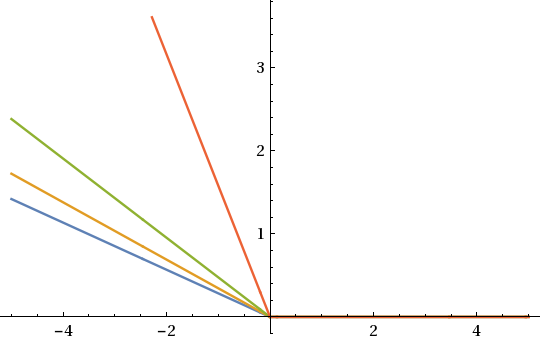
\includegraphics[width=.45\textwidth]{breaking.png}
\caption{Решение $u(t,x)$ типа <<неподвижный фронт>> в последовательные моменты времени (справа) в случае $k = 2, x_0 = 0$}
\end{figure}

\end{document}
